
\begin{frame}{\appendixname~\theappendixframenumber~: Non-linear problems}\labelappendixframe{frame:nonlinear}
	TODO
\end{frame}
\addtocounter{appendixframenumber}{1}

\section{\appendixname~\theappendixframenumber~: Data-driven vs Physics-Informed training}\labelappendixframe{frame:datavspinns}

\begin{frame}{\appendixname~\theappendixframenumber~: Problem considered}
	\textbf{Problem statement:} Consider the Poisson problem in 1D with Dirichlet BC:
	\vspace{-5pt}
	\begin{equation*}
		\left\{
		\begin{aligned}
			-\partial_{xx} u & = f, \; &  & \text{in } \; \Omega \times \mathcal{M}, \\
			u         & = 0, \;  &  & \text{on } \; \partial\Omega \times \mathcal{M},
		\end{aligned}
		\right.
		% \label{eq:Lap2D}\tag{$\mathcal{P}$}
	\end{equation*}

	\vspace{-5pt}
	with $\Omega=[0,1]^2$ and $\mathcal{M}=[0,1]^3$ ($p=3$ parameters).
		
	\vspace{4pt}
	\textbf{Analytical solution :} $\quad u(x;\bm{\mu})=\mu_1\sin(2\pi x)+\mu_2\sin(4\pi x)+\mu_3\sin(6\pi x) \,.$

	\vspace{4pt}
	\textbf{Construction of two priors:} MLP of 6 layers; Adam optimizer (10000 epochs). \\
	Imposing the Dirichlet BC exactly in the PINN with $\varphi(x)=x(x-1)$.

	\begin{itemize}
		\item \textbf{Physics-informed training:} $N_\text{col}=5000$ collocation points.
		$$J_r(\theta) \simeq
			\frac{1}{N_\text{col}} \sum_{i=1}^{N_\text{col}} \big| \partial_{xx}u_\theta(\bm{x}_\text{col}^{(i)};\bm{\mu}_\text{col}^{(i)}\big) + f\big(\bm{x}_\text{col}^{(i)};\bm{\mu}_\text{col}^{(i)}\big) \big|^2.$$
	
		\item \textbf{Data-driven training:}  $N_\text{data}=5000$ data.
		$$J_\text{data}(\theta) =
		\frac{1}{N_\text{data}}
		\sum_{i=1}^{N_\text{data}} \big| u_\theta^\text{data}(\bm{x}_\text{data}^{(i)};\bm{\mu}_\text{data}^{(i)}) - u(\bm{x}_\text{data}^{(i)};\bm{\mu}_\text{data}^{(i)}) \big|^2.$$
	\end{itemize}
\end{frame}

\begin{frame}{Priors derivatives}
	\vspace{-10pt}
	$$\bm{\mu}^{(1)}=(0.3,0.2,0.1)$$
	\begin{figure}[ht!]
		\centering
		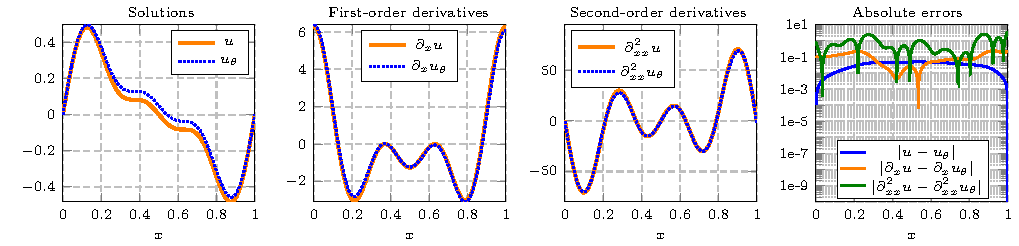
\includegraphics[width=\linewidth]{images/appendix/datavspinns/standalone_solutions_and_errors_PINN.pdf}
	\end{figure}
	
	\begin{figure}[ht!]
		\centering
		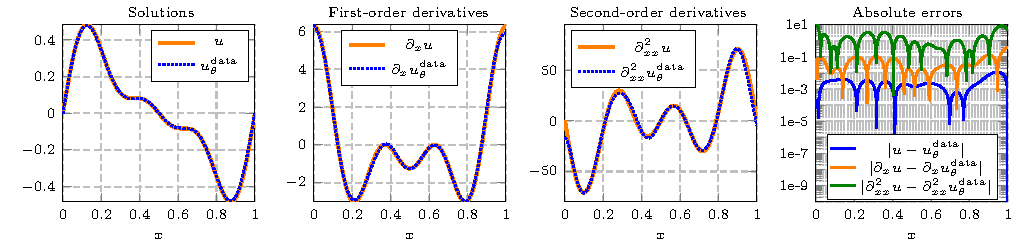
\includegraphics[width=\linewidth]{images/appendix/datavspinns/standalone_solutions_and_errors_NN.pdf}
	\end{figure}
\end{frame}

\begin{frame}{Additive approach in $\mathbb{P}_1$}
	\vspace{-2pt}
	\textbf{1 set of parameters:} $\quad \bm{\mu}^{(1)}=(0.3,0.2,0.1)$
	
	\begin{table}[H]
		\centering
		\gainsbothNN{images/appendix/datavspinns/FEM_param1.csv}{images/appendix/datavspinns/compare_gains_param1.csv}
	\end{table}

	\vspace{6pt}
	\textbf{50 set of parameters:}

	\begin{table}[H]
		\centering
		\gainstableMult{images/appendix/datavspinns/Tab_stats_case1_degree1.csv}
	\end{table}

	\footnotesize
	$N$ : Nodes.
\end{frame}

\addtocounter{appendixframenumber}{1}

\section{\appendixname~\theappendixframenumber~: Multiplicative approach}\labelappendixframe{frame:mult}

\begin{frame}{\appendixname~\theappendixframenumber~: Multiplicative approach}
	TODO
\end{frame}
\addtocounter{appendixframenumber}{1}